\section{ Joukkueen kokoaminen ja tavoitteet }
\label{4-way-joukkuehyppaaminen-joukkueen-kokoaminen-ja-tavoitteet}


Joukkueen kokoamisessa huomioon otettavia asioita ovat jäsenten kokemus, tavoitteet ja halu/valmius harjoitteluun. Kokemustaso joukkueessa voi vaihdella paljonkin, mutta tavoitteiden on oltava samansuuntaiset. Tavoitteiden yhteisellä asettelulla saadaan joukkueella harjoittelemisesta paras hyöty. Tavoitteena voi olla esim. kisoihin osallistuminen, tietty pistekeskiarvo, hauskaa hyppäämistä yhdessä tai monen vuoden määrätietoinen harjoittelu. 


Yleisten joukkueen tavoitteiden lisäksi jokaisella jäsenellä voi olla omia tavoitteita, esim. lentoasennon parantaminen. 


Hyvä joukkue ei välttämättä synny lahjakkaista yksilöistä, vaan se vaatii jokaiselta jäseneltä yhtä suurta sitoutumista ja sopeutumista, kykyä toimia ryhmässä yhteisen edun hyväksi. 


Joukkueen suurin voimavara on hyvä yhteishenki. Yhteisten tavoitteiden asettaminen ja niihin määrätietoisesti pyrkiminen luovat perustan koko joukkueen kehittymiselle. 


\begin{Figure}\centering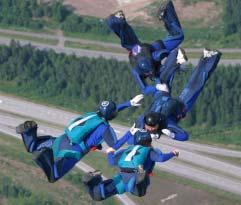
\includegraphics[width=0.7\textwidth]{Neliway-ilmassa.jpeg}\captionof{figure}{4-way -joukkue ilmassa}\end{Figure} 

\section{ Joukkueen jäsenet }
\label{4-way-joukkuehyppaaminen-joukkueen-jasenet}


Jokaisella joukkueen jäsenellä on oma paikka sekä tehtävä. Karkeasti joukkueen voi jakaa keskustaan ja fluttereihin. Keskustatyöskentely vaatii täsmällisyyttä ja tarkkuutta. Keskusta määrittää muodostelman keskipisteen ja suunnan, jonka suhteen flutterit työskentelevät. Fluttereiden on pystyttävä työskentelemään nopeasti ja joustavasti suhteessa keskustaan. Toisin sanoen keskustan epätarkkuus kertautuu pidempänä matkana fluttereille. 


Tarkemmat tehtävät määräytyvät uloshyppypaikkojen mukaan: 


\begin{Figure}\centering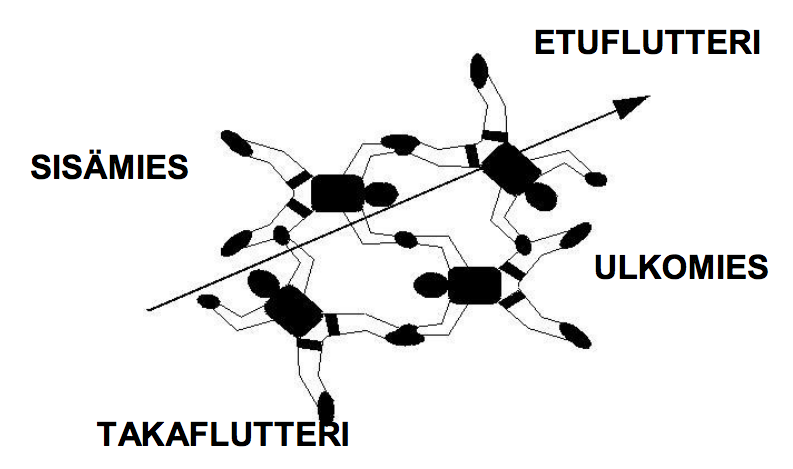
\includegraphics[width=0.95\textwidth]{4-way-paikat.png}\captionof{figure}{4-way joukkueen uloshyppypaikat}\end{Figure} 


Kuvassa lentokoneen lentosuunta on merkitty nuolella. Uloshyppy toimii samalla tavoin riippumatta siitä, kummalla puolella lentokonetta ovi on.  

\begin{description}
\item[Sisämies ] \hfill \\ 
Kontrollikeskus, suurin osa puruista, eniten otteita. \hfill \\ 
\end{description}
\begin{description}
\item[Ulkomies, ripustin ] \hfill \\ 
Osa puruista, pidempiä liikkeitä ja käännöksiä kuin sisämiehellä. \hfill \\ 
\end{description}
\begin{description}
\item[Etuflutteri ] \hfill \\ 
Ei näe kaikkea, joutuu työskentelemään enemmän tuntumalla kuin katseella. \hfill \\ 
\end{description}
\begin{description}
\item[Takaflutteri ] \hfill \\ 
Näkee paljon, pitkiä liikkeitä, vaatii joustavuutta. \hfill \\ 
\end{description}
\begin{description}
\item[Videokuvaaja ] \hfill \\ 
Kuvaa joukkueen suorituksen, joko harjoittelua varten tai kilpailuissa tuomarointia varten. \hfill \\ 
\end{description}
\begin{description}
\item[Varamies ] \hfill \\ 
Paikkaa tarvittaessa. Monitaituri. \hfill \\ 
\end{description}

Etuflutteri ja ulkomies muodostavat \textit{etupuljan} ja takaflutteri ja sisämies \textit{takapuljan.} Suurin osa blokkien siirtymistä vaatii työskentelyä puljittain. Muutamissa blokeissa välisuorituksen tekevät yksittäinen hyppääjä ja kolmen pulja. 

\section{ Valmentaja }
\label{4-way-joukkuehyppaaminen-valmentaja}


Joukkueen kannattaa jo kokoamisvaiheessa hankkia valmentaja. Varsinkin harjoittelun alkuvaiheessa valmentajan avustuksella pystytään välttämään paljon ongelmia ja virheitä, joita saattaa syntyä pelkästään omin avuin miettimällä. Joukkueen tasosta riippuu, minkälaista valmennusta tarvitaan. Aloitteleva joukkue tarvitsee valmentajan, joka osaa opettaa perusasiat ja random- sekä blokkitekniikoiden perusteet. Valmentajan tehtäviin kuuluu myös videoiden analysointia, hyppyjen suunnittelua ja lautakuivien ohjaamista. Varsinkin harjoittelun alussa valmentaja osaa antaa harjoitukselle suuntaa ja pureutua ongelmakohtiin. Valmentaja pystyy myös selvittämään ongelmia/näkemyseroja, joita joukkue ei välttämättä keskenään osaa ratkaista 

